\subsection{Experiment 2: Metric Relations}

\begin{figure}
    \centering
    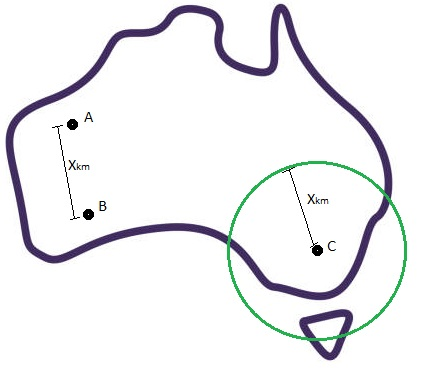
\includegraphics[width=0.3\textwidth]{figures/metric_AUS_diagram.jpg}
    \caption{Visual depiction of the metric relation task corresponding to Prompts 3-5. Given a pair of reference entities $A$ and $B$, and a query entity $C$, the LLM is prompted to retrieve an entity with a metric distance from $C$ as similar as possible to the metric distance between $A$ and $B$. Entities falling on the green circle represent the best responses to the question.}
    \label{fig:metric-AUS-diagram}
\end{figure}

To determine if LLMs can reason about metric (distance) spatial relations, we devise three types of prompts, each asking to retrieve places based on implicit quantitative metric relationships.
%
The general problem is, given a reference pair of cities, $A$ and $B$ that are separated by a distance of $x$, and a query city $C$, the task is to retrieve a fourth city whose distance from $C$ is as close to $x$ as possible.
Since we aim to test for implicit metric reasoning, rather than stating the distance $x$ explicitly, we prompt the LLM for a city whose distance from $C$ is similar to the distance between $A$ and $B$.
The task is depicted visually in Figure \ref{fig:metric-AUS-diagram}, where the ideal response will be the name of a city whose geocoordinates fall on or near the perimeter of the circle.
The following `neutral' prompt is the first of the three variants we use to elicit responses from the models:

\begin{lstlisting}[title=Prompt 3: Neutral Metric Prompt]
    The distance from A to B is similar to the distance from C to what other city or town?
\end{lstlisting}

\noindent Based on previous work~\cite{Bhandari2023}, LLMs have been shown to retrieve places that are closer to a query location when the prompt includes the keyword `near', and retrieve places that are farther from the query location when the keyword `far' is used in the prompt.
To further examine this idea we devise two variants of the neutral metric prompt.
By introducing the keyword `near' or `far' into the prompt, we aim to measure if LLMs have a static representation of those keywords, or if they can adapt the meaning of `near' or `far' based on the scale of the question.
The `near' and `far' prompts are as follows:

\begin{lstlisting}[title=Prompt 4: `Near' Metric Prompt]
    If A is 'near' to B, what is a city or town 'near' to C?
\end{lstlisting}

\begin{lstlisting}[title=Prompt 5: `Far' Metric Prompt]
    If A is 'far' from B, what is a city or town 'far' from C?
\end{lstlisting}



\noindent We populate the prompts with cities and towns of varying populations sampled from across the states and territories of Australia, including both indigenous and western place names.
We measure the geodesic distance between the place returned by the LLM and the query location $C$ and report this as \texttt{predicted{\_}distance}.
In the ideal case, the \texttt{predicted{\_}distance} will match closely to the distance $x$, which we report as the \texttt{target{\_}distance}.
Both distances are normalized by the approximate diameter of the country, so that error tolerance scales with $x$.



\subsection{Result 2. Metric Relations}

Figure \ref{fig:metric-plots} shows the results of Experiment 2.
Across all three prompt types, the distances between the places returned by the models and the query points (\texttt{predicted{\_}distances)} were not similar to the distances between the reference places provided in the prompt (\texttt{target{\_}distances}).
In many cases, the distances were too large or too small by thousands of Kilometers.
%
Given prompts where the implicit \texttt{target{\_}distance} is considered `near' (`far') and asking for a place `near' to (`far' from) the query point, the models consistently chose places too close to (far from) the query point.
This was especially pronounced for the keyword `near', which resulted in places returned that were never further than 1,000 Kilometers from the query point, no matter how far the implicit \texttt{target{\_}distance} was (up to 4,000 Kilometers in some prompts).



\begin{figure*}[h]
    \centering
    \subfigure[Target distance vs. predicted distance for `far' metric prompt. Three outliers with extremely high predicted distances are omitted, along with 100 abstentions out of 280 model responses.]{
        \includesvg[width=0.3\textwidth]{figures/metric_scatter_far}
        \label{fig:metric-plot-far}
    }
    \hfill
    \subfigure[Target distance vs. predicted distance for neutral metric prompt. Four outliers with extremely high predicted distances are omitted, along with 159 abstentions out of 280 model responses.]{
        \includesvg[width=0.3\textwidth]{figures/metric_scatter_neutral}
        \label{fig:metric-plot-neutral}
    }
    \hfill
    \subfigure[Target distance vs. predicted distance for `near' metric prompt. Eleven outliers with extremely high predicted distances are omitted, along with 89 abstentions out of 280 model responses.]{
        \includesvg[width=0.3\textwidth]{figures/metric_scatter_near}
        \label{fig:metric-plot-near}
    }
    \caption{Results of three metric relation prompts: `far', neutral, and `near'. Target distance represents the distance between `A' and `B' in Prompts 3-5, and predicted distance represents the distance between `C' and the place returned by the model. Points closer to the line drawn at $y = x$ represent more accurate metric spatial reasoning than points further from that line.}
    \label{fig:metric-plots}
\end{figure*}


% \begin{figure*}[h]
%     \centering
%     \begin{subfigure}[t]{\textwidth}
%         \includesvg[width=.25\textwidth]{figures/metric_scatter_far}
%         % \caption{\small A candidate location X has named objects A-D with the spatial layout depicted above.} 
%         \label{fig:CM-LO-Example}
%     \end{subfigure}
%     \hfill
%     \begin{subfigure}[t]{\textwidth}
%         \includesvg[width=.25\textwidth]{figures/metric_scatter_neutral}
%         % \caption{\small The objects are binned into spatial quadrants based on their relative position to the location coordinates, X.} 
%         \label{fig:CM-LO-Setup}
%     \end{subfigure}
%     \hfill
%         \begin{subfigure}[t]{\textwidth}
%         \includesvg[width=.25\textwidth]{figures/metric_scatter_near}
%         % \caption{\small Rank the locations by the number of query terms found in the correct quadrant for the location.}
%         \label{fig:CM-LO-Query}
%     \hfill
%     \end{subfigure}
%     \caption{\textbf{Location-Object Search Method. A Location-Object data structure (Figure \ref{fig:CM-LO-Setup}) is generated based on the cardinal relations between the objects and the location (Figure \ref{fig:CM-LO-Example}). Then a pictorial query is matched against the structure (Figure \ref{fig:CM-LO-Query}).}}\label{figure:ConceptMap-LO} 
% \end{figure*}





\subsection{Metric Relations}

\citeauthor{Bhandari2023} prompt the LLMs to generate names of cities that are ``near'' or ``far'' from a provided reference city.
They show that the resulting cities generated tend to be closer in distance to the reference point when the ``near'' prompt is used, and farther when the ``far'' prompt is used, indicating LLMs associate a smaller metric (distance) to the word `near' than to the word `far'~\cite{Bhandari2023}.
Our results show that these keywords are associated with static distances (i.e. everything `near' a query point was within 1,000 Kilometers of it) even despite prompting that implicitly contained a scale for what `near' should mean (such as a pair of reference cities that were 1,500 Kilometers apart).
All models tested showed this bias towards relying on the qualitative keyword hints in the prompt (`near' or `far') rather than performing quantitative metric reasoning to retrieve places the correct distance to the query point.
The neutral prompt that contained no keyword hint did not show a bias towards too large or small distances, but the spread indicates that the places retrieved were not very close to the correct distance (often off by a thousand or more Kilometers).
